\subsection{Ionic Bond}
\begin{minipage}{0.55\linewidth}
    $\circ$ Ions held together by electrostatic attraction\\
    $\circ$ Metal loses VE, non-metal gains VE\\
    $\circ$ Strength quantified by lattice energy\\
    $\circ$ Bond is considered ionic if $\Delta EN > 2.0$\\
    \vspace{1pt}\\
    \textbf{Some Definitions}\\
    \textbf{Ionization Energy}: energy required to ionize (remove) $e^-$ from atom or ion\\
    \textbf{Electron Affinity}: energy change when adding and extra $e^-$ to an atom (typically exothermic)\\
    \textbf{Lattice Energy}: energy required to separate ions in ionic solid to infinite distance 
\end{minipage}
\begin{minipage}{0.44\linewidth}
    \begin{center}
        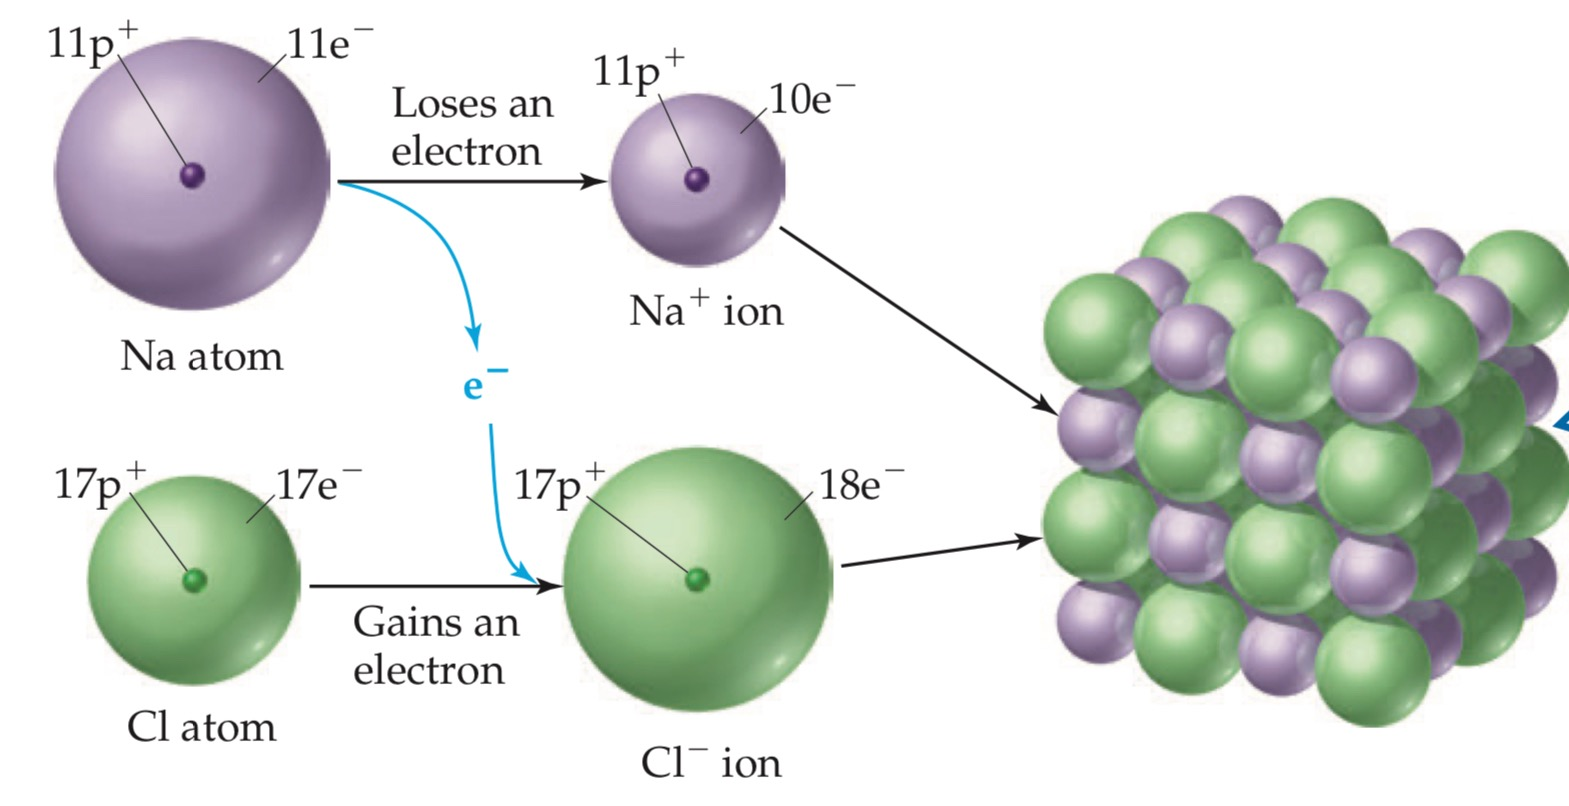
\includegraphics[width = 0.9\linewidth]{images/NaCl.jpeg}
    \end{center}
\end{minipage}\\
\vspace{1pt}\\
\textbf{Bookkeeping Systems}\\
\begin{center}
  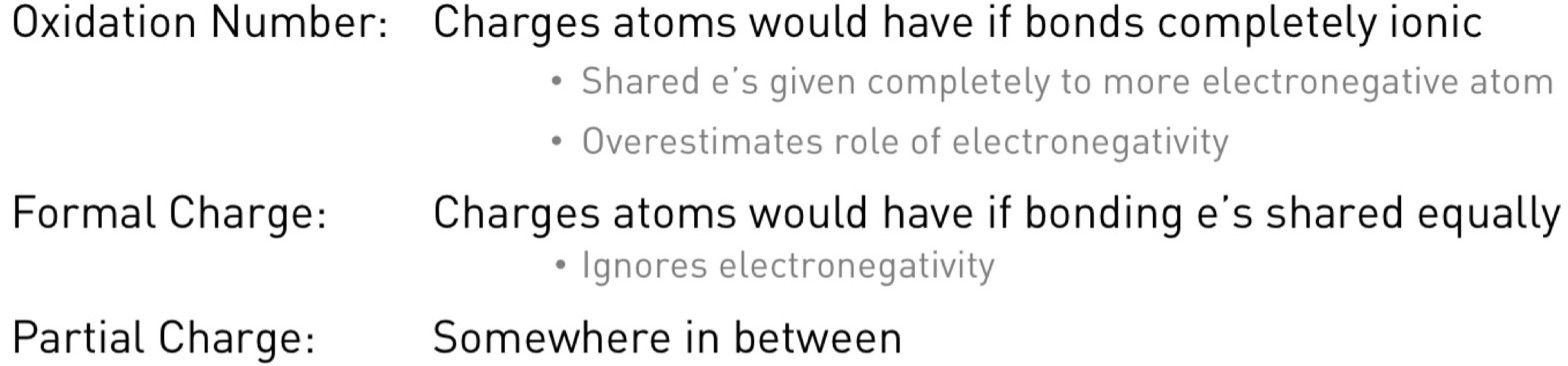
\includegraphics[width = 0.7\linewidth]{images/Bookkeeping_Systems.jpeg} 
\end{center}
\textbf{Oxidation Numbers}\\
\begin{center}
  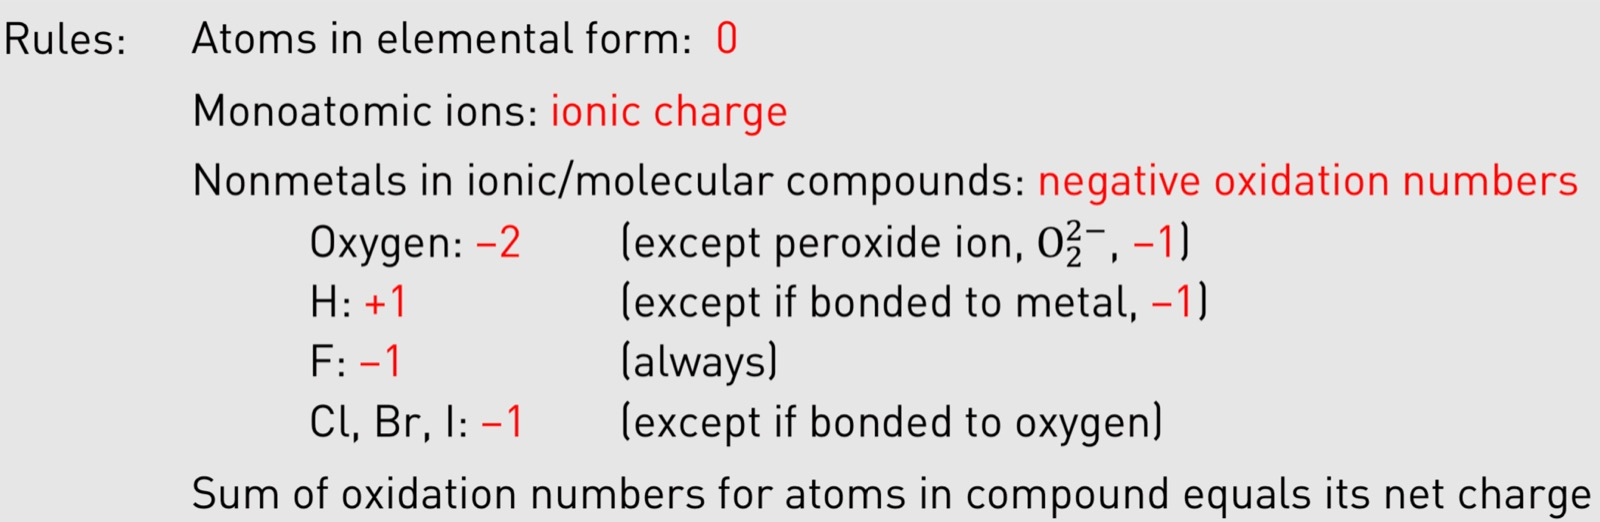
\includegraphics[width = 0.95\linewidth]{images/Oxidations_Numbers.jpeg} 
\end{center}
\textbf{Lattice Energy (e.g NaCl)}\\
\begin{minipage}{0.6\linewidth}
\begin{center}
   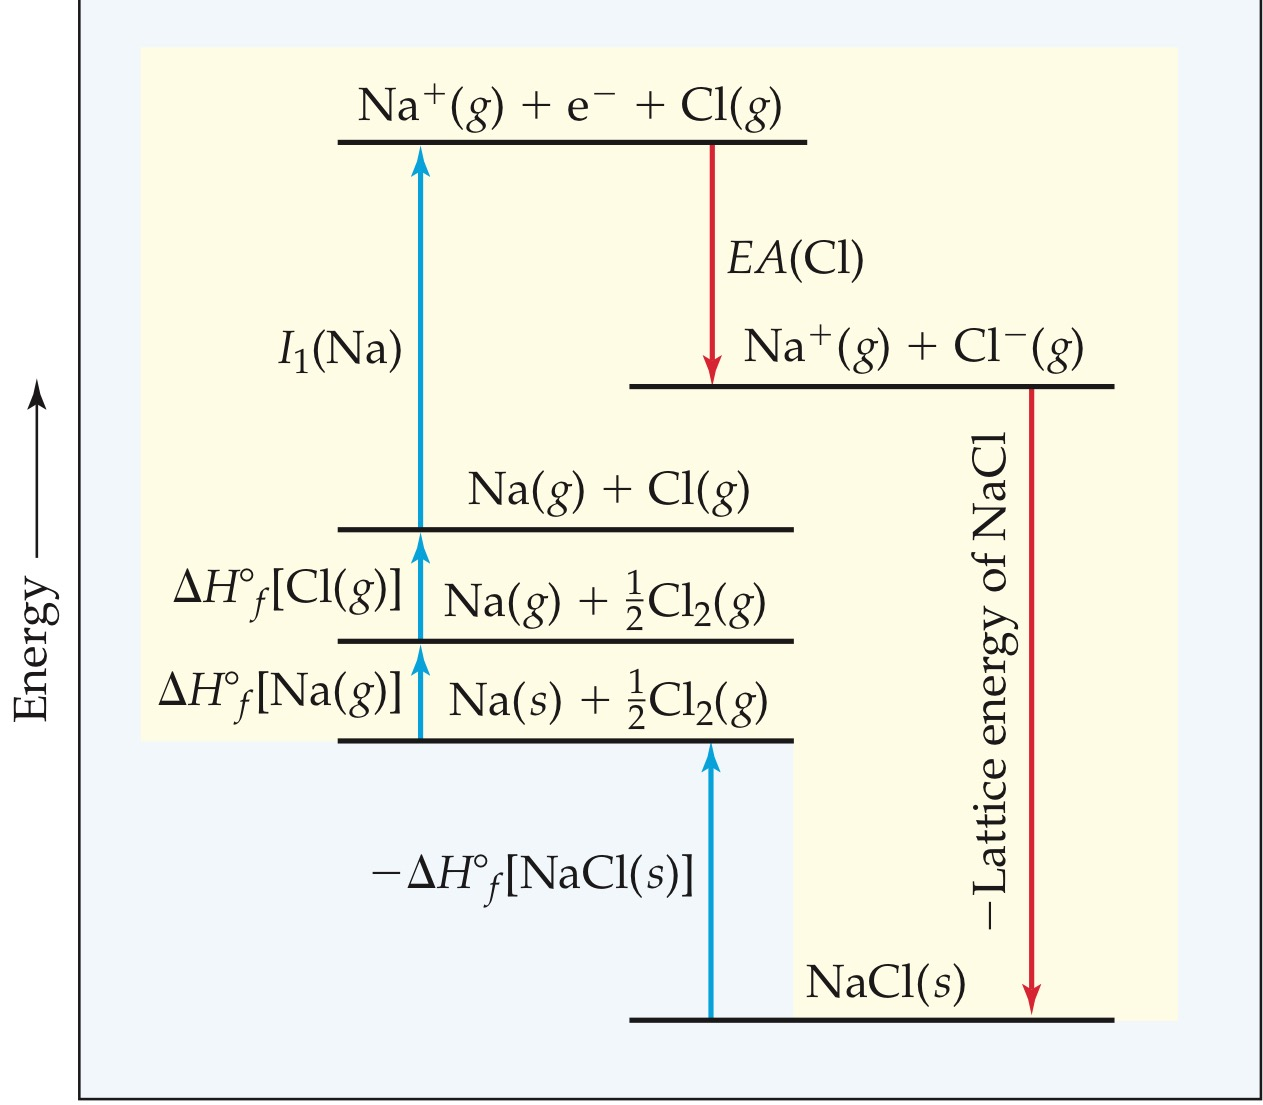
\includegraphics[width = 0.8\linewidth]{images/Lattice_Energy_NaCl.jpeg}     
\end{center}

\end{minipage}
\begin{minipage}{0.39\linewidth}
\begin{center}
    {\normalsize $\Delta H_{lattice}$ \\
    $= - \Delta H_f^{\circ}[NaCl(s)]$ \\
    $+ \Delta H_f^{\circ}[Na(g)]$\\
    $+ \Delta H_f^{\circ}[Cl(g)]$\\
    $+ I_1[Na]$\\
    $+ EA[Cl]$}
\end{center}
   
\end{minipage}

